\documentclass{acmsiggraph}                     % final
%\documentclass[annualconference]{acmsiggraph}  % final (annual conference)
%\documentclass[review]{acmsiggraph}            % review
%\documentclass[widereview]{acmsiggraph}        % wide-spaced review
%\documentclass[preprint]{acmsiggraph}          % preprint

%% Uncomment one of the five lines above depending on where your paper is
%% in the conference process. ``review'' and ``widereview'' are for review
%% submission, ``preprint'' is for pre-publication, and ``final'' is for
%% the version to be printed. The ``final'' variant will accept the 
%% ``annualconference'' parameter, which changes the height of the space
%% left clear for the ACM copyright information.

%% The 'helvet' and 'times' packages define the typefaces used for
%% serif and sans serif type in this document. Computer Modern Roman 
%% is used for mathematics typesetting. The scale factor is set to .92
%% to bring the sans-serif type in line with the serif type.

\usepackage[scaled=.92]{helvet}
\usepackage{times}

%% The 'graphicx' package allows for the inclusion of EPS figures.

\usepackage{graphicx}

%% use this for zero \parindent and non-zero \parskip, intelligently.

\usepackage{parskip}

%% Optional: the 'caption' package provides a nicer-looking replacement
%% for the standard caption environment. With 'labelfont=bf,'textfont=it',
%% caption labels are bold and caption text is italic.

\usepackage[labelfont=bf,textfont=it]{caption}

%% If you are submitting a paper to the annual conference, please replace 
%% the value ``0'' below with the numeric value of your OnlineID. 
%% If you are not submitting this paper to the annual conference, 
%% you may safely leave it at ``0'' -- it will not be included in the output.

\onlineid{0}

%% Paper title.

\title{News Knitter}

%% Author and Affiliation (single author).

%%\author{Roy G. Biv\thanks{e-mail: roy.g.biv@aol.com}\\Allied Widgets Research}

%% Author and Affiliation (multiple authors).

\author{Ebru Kurbak\thanks{e-mail:ebru.kurbak@ufg.ac.at}\\ University of Art and Industrial Design Linz %
\and Mahir M. Yavuz\thanks{e-mail:mahir.yavuz@ufg.ac.at}\\University of Art and Industrial Design Linz}

%% Keywords that describe your work.

\keywords{radiosity, global illumination, constant time}

%%%%%% START OF THE PAPER %%%%%%

\begin{document}

\teaser{
  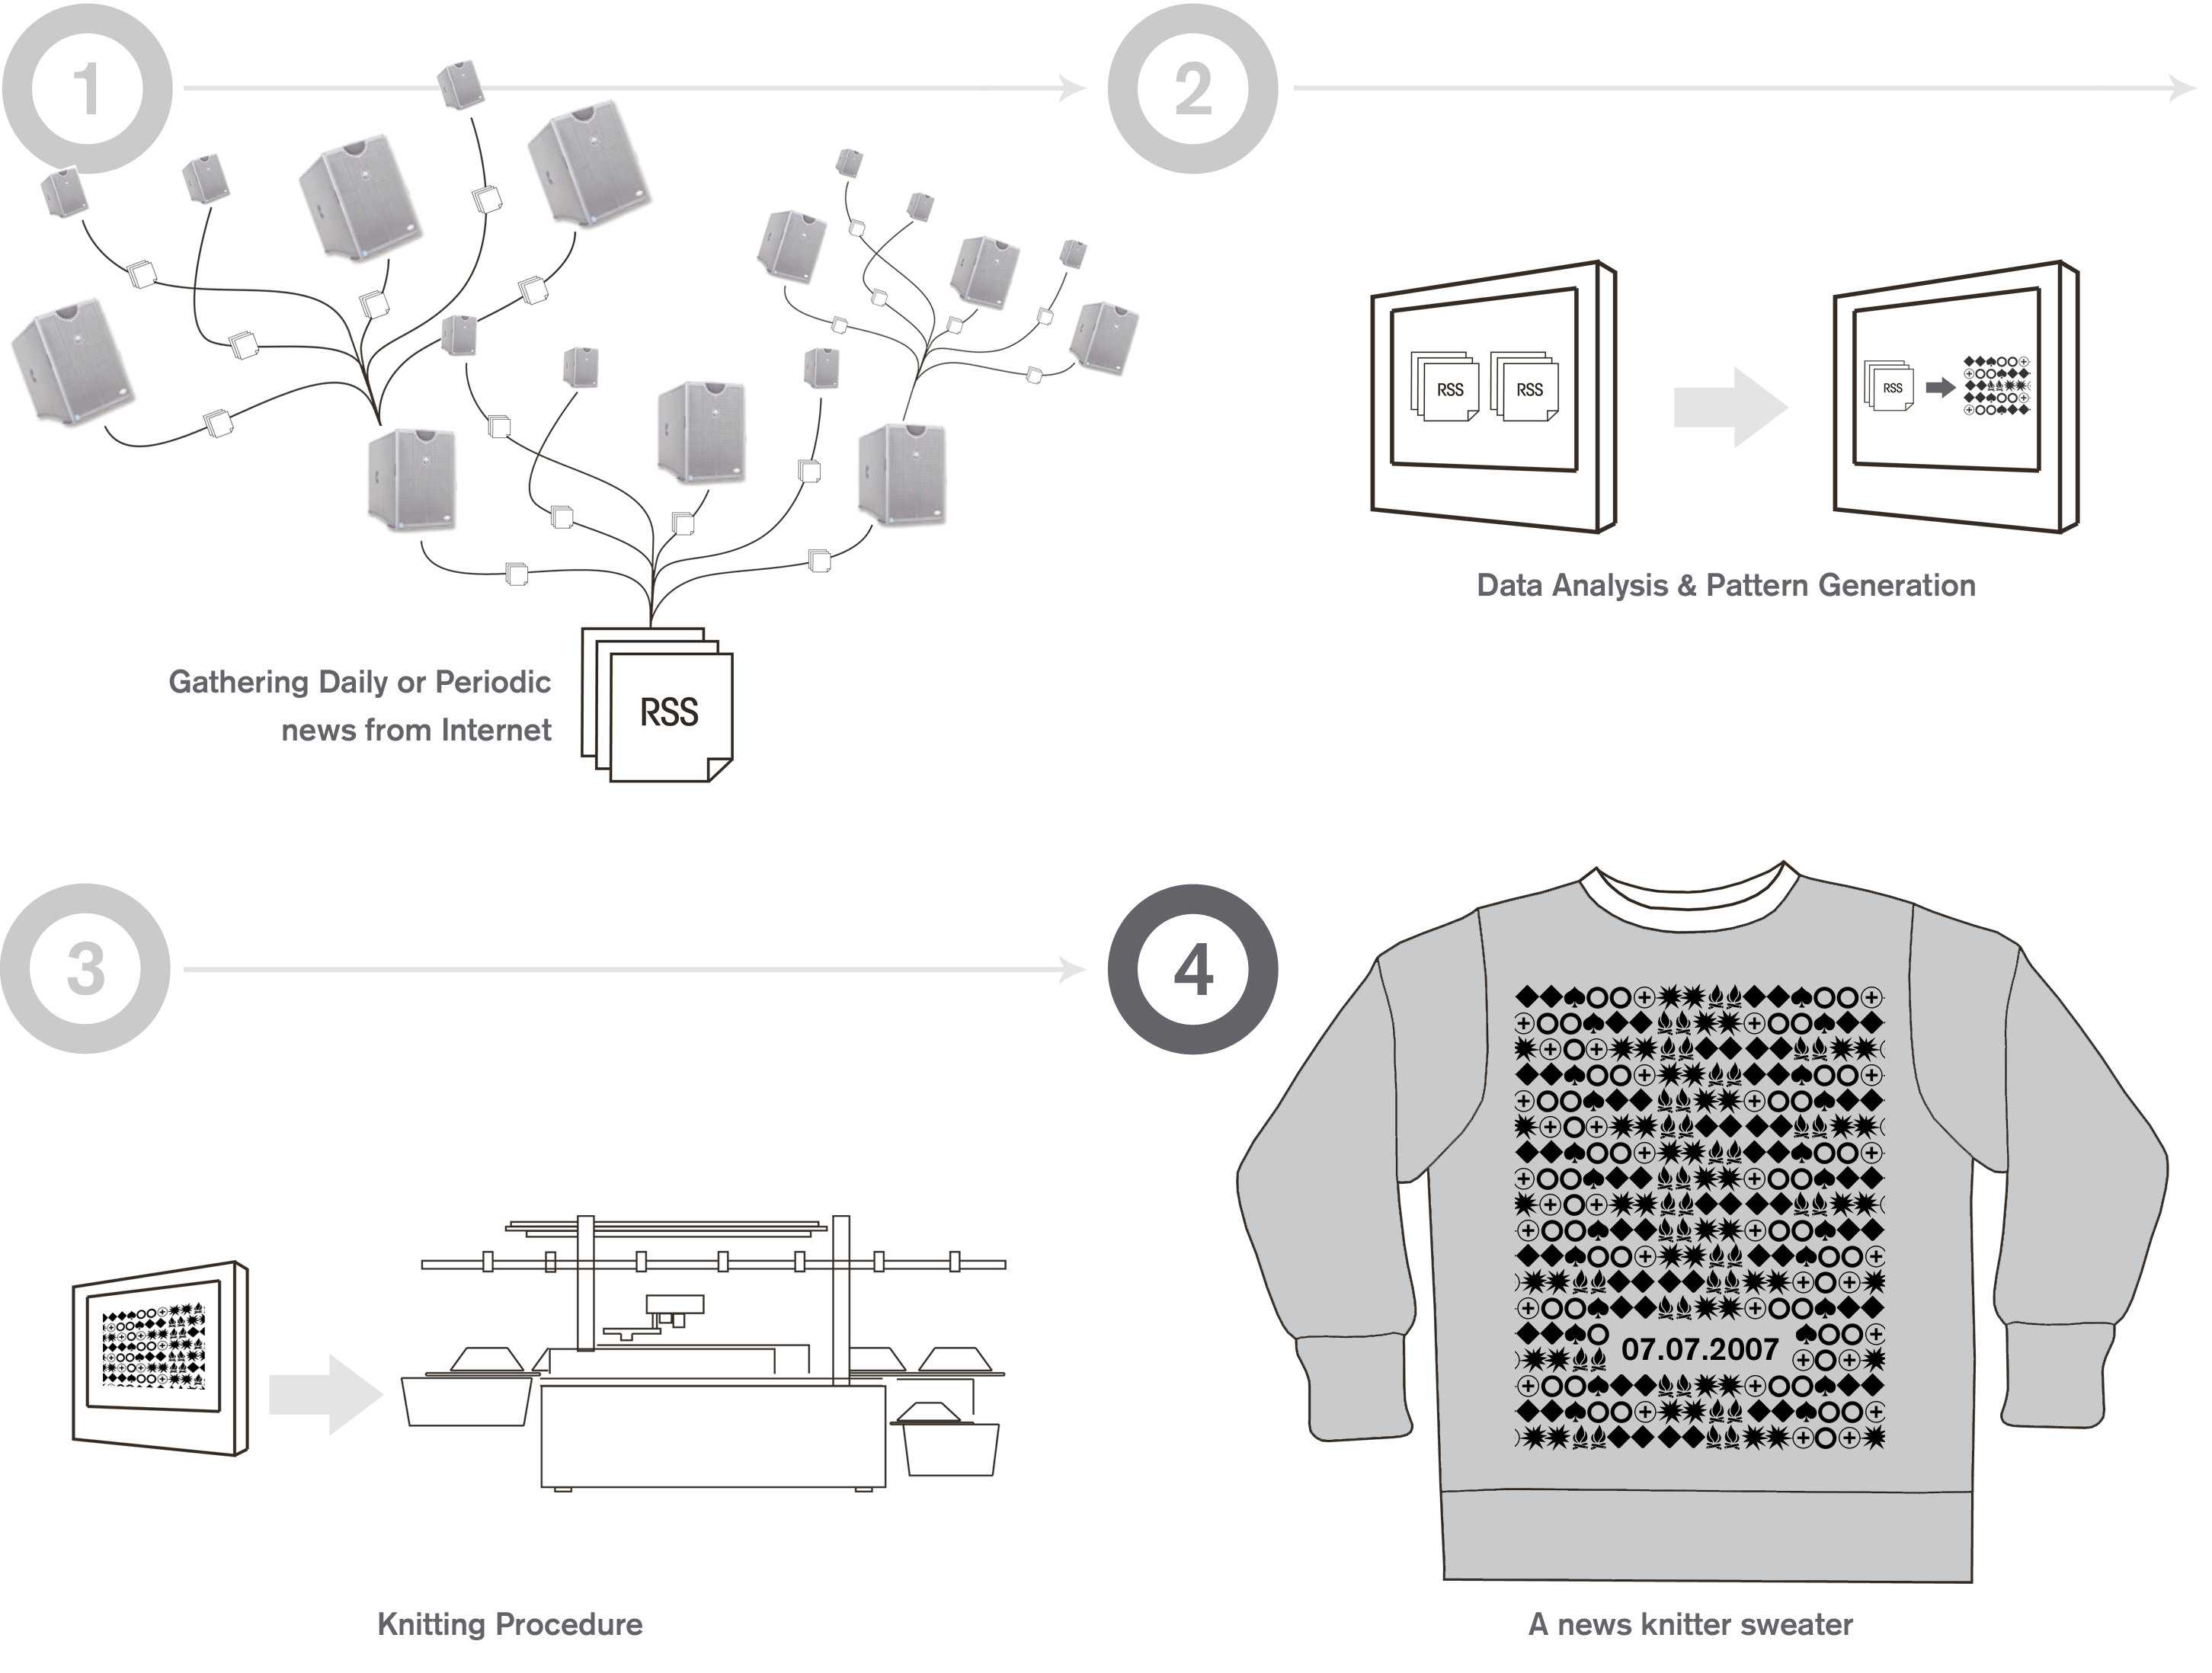
\includegraphics[width=4in]{00-nk-diagram.png}
  \caption{News Knitter Production Flow}
}

%% The ``\maketitle'' command must be the first command after the
%% ``\begin{document}'' command. It prepares and prints the title block.

\maketitle

%% Abstract section.

%% \begin{abstract}

%% Duis autem vel eum iriure dolor in hendrerit in vulputate velit esse
%% molestie consequat, vel illum dolore eu feugiat nulla facilisis at 
%% vero eros et accumsan et iusto odio dignissim qui blandit praesent
%% luptatum zzril delenit augue duis dolore te feugait nulla
%% facilisi. Lorem ipsum dolor sit amet, consectetuer adipiscing elit,
%% sed diam nonummy nibh euismod tincidunt ut laoreet dolore magna
%% aliquam erat volutpat.

%% Citations can be done this way~\cite{Jobs95} or this more concise 
%% way~\shortcite{Jobs95}, depending upon the application.

%% Ut wisi enim ad minim veniam, quis nostrud exerci tation ullamcorper
%% suscipit lobortis nisl ut aliquip ex ea commodo consequat. Duis autem
%% vel eum iriure dolor in hendrerit~\cite{Pellacini:2005:LAH}
%% in vulputate velit esse molestie~\cite{notes2002} 
%% consequat, vel illum dolore eu feugiat nulla facilisis at vero eros et
%% accumsan et iusto odio dignissim qui blandit praesent luptatum zzril
%% delenit augue duis dolore te feugait nulla facilisi.~\cite{Park:2006:DSI}

%% \end{abstract}

%% ACM Computing Review (CR) categories. 
%% See <http://www.acm.org/class/1998/> for details.
%% The ``\CRcat'' command takes four arguments.

%% \begin{CRcatlist}
%%   \CRcat{K.6.1}{Management of Computing and Information Systems}%
%% {Project and People Management}{Life Cycle};
%%   \CRcat{K.7.m}{The Computing Profession}{Miscellaneous}{Ethics}
%% \end{CRcatlist}

%% The ``\keywordlist'' command prints out the keywords.
%% \keywordlist

\section{Introduction}

%% The ``\copyrightspace'' command must be the first command after the 
%% start of the first section of the body of your paper. It ensures the
%% copyright space is left at the bottom of the first column on the first
%% page of your paper.

%% \copyrightspace

News Knitter is an information visualization project which materializes ephemeral online data through wearable garments. Large scale data gathered from online political news is used as a source to generate patterns for a fully computerized knitting machine. Knitting, which is a very conventional mode of physical production, is preferred as a medium to embody digital information and to produce daily, wearable, washable sweaters. Digital bits are transformed into physical stitches and the information is visualized through three dimensional, tactile, personal belongings. 


\section{Exposition}

Starting from the prehistoric practice of producing nets and basketry, the textile industry has always improved its production techniques for the purpose of increasing efficiency. The introduction of machinery into the industry, and subsequently the development of the fully automatic systems of textile machinery has increased the volume of production drastically. Today, contemporary trends of fabrication of clothing utilize computers and high-technology at a variety of steps of the process. Knitted garments, in particular, are produced with highly complex and fully computerized knitting machines in both industrialized and developing countries. These machines allow much more flexibility in terms of patterning compared to the previous modes of knitting. Today, any digital raster image can be converted into a proper pattern for knitting by the patterning software. However, the patterning of knitted garments is still seen as a design problem of an individual and altogether handled by pattern technicians manually, if not sketched by a fashion designer. News Knitter proposes an innovative workflow and production pipeline as an alternative for the common methods of fabrication of knitted garments. It translates the individual design process of patterning into a world-wide collaboration by utilizing live data streams as a source for pattern generation. Real-time news data and meta-data related to daily global news items are captured, analyzed and filtered into functional sets of data. The data is then used to generate visuals which are compatible with the patterning software of a fully computerized knitting machine. Due to the dynamic nature of live data streams, the elements of global participation and unpredictability are introduced into the design process. 

Each product, sweater of News Knitter is an evidence of a specific day or period. The pre-defined software algorithms shape the input data and generate a unique pattern. As a result, an unpredictable unique message is delivered through a particular pattern which employs each person who wears a News Knitter sweater to carry and spread a unique message.

\section{Conclusion}

Situated on the thresholds of digital data visualization and analog convention of knitting, News Knitter offers a fresh insight to new modes of industrial production. It brings the two controversial concepts, unique design and mass production, into discussion. Furthermore, the methods employed in News Knitter may enable a more customized and personalized way of pattern generation which would allow any user to interrupt the process of mass production at any time. The patterns could be generated according to person specific dates, such as birthdays and anniversaries, or by using a personal data source such as personal blog posts, twitter updates, last.fm statistics and facebook status messages. Even users could be able to upload their own private data sheets, such as their credit card history, their own voice graphs and create their desired unique knitted garments. 


\bibliographystyle{acmsiggraph}
\nocite{*}
\bibliography{template}
\end{document}
